\documentclass{beamer}

\usepackage[utf8]{inputenc}
\usepackage{default}
\usepackage{amssymb,amsmath,amsfonts}
\usepackage{graphicx}
\usepackage{color}
%\usepackage{colortbl}
%\usepackage{todonotes}
\usepackage{hyperref}
\usepackage{cleveref}
%\usepackage{subfig}
\usepackage{bm}
%\usepackage{listings}
\usepackage{multimedia}
%\usepackage{media9}
%\usepackage{multirow}
%\usepackage{cite}
\usepackage[round]{natbib}   % omit 'round' option if you prefer square brackets
\bibliographystyle{plainnat}

\newcommand{\highlight}[1]{%
  \colorbox{red!50}{$\displaystyle#1$}}
  
  \newcommand{\x}{\mathbf{x}}
\newcommand{\y}{\mathbf{y}}
\newcommand{\q}{\boldsymbol{\theta}}
\newcommand{\io}{\int_\Omega}
\newcommand{\ve}{\varepsilon}
\newcommand{\pa}{\partial}

\newcommand{\F}{\mathbf{F}}

\newcommand{\highlightcustom}[2][yellow]{\mathchoice%
  {\colorbox{#1}{$\displaystyle#2$}}%
  {\colorbox{#1}{$\textstyle#2$}}%
  {\colorbox{#1}{$\scriptstyle#2$}}%
  {\colorbox{#1}{$\scriptscriptstyle#2$}}}%

\mode<presentation>
{
    \usetheme{Madrid}
    \usecolortheme{rose}
}
  
\title[Scalar Reduction of a Neural Field]{Scalar Reduction of a Neural Field Model with Spike Frequency Adaptation} % The short title appears at the bottom of every slide, the full title is only on the title page

\author[Y. Park \& G.B. Ermentrout]{Youngmin Park \& Bard Ermentrout} % Your name
\institute[U Pitt]% Your institution as it will appear on the bottom of every slide, may be shorthand to save space
{
University of Pittsburgh Department of Mathematics\\ % Your institution for the title page
\medskip
\textit{yop6@pitt.edu} % Your email address
}
\date{\today} % Date, can be changed to a custom date

% show page number
\addtobeamertemplate{navigation symbols}{}{%
    \usebeamerfont{footline}%
    \usebeamercolor[fg]{footline}%
    \hspace{1em}%
    \insertframenumber/\inserttotalframenumber
}

\begin{document}

\begin{frame}
\titlepage % Print the title page as the first slide
\end{frame}
% 
% \begin{frame}
% \frametitle{Overview} % Table of contents slide, comment this block out to remove it
% \tableofcontents % Throughout your presentation, if you choose to use \section{} and \subsection{} commands, these will automatically be printed on this slide as an overview of your presentation
% \end{frame}

%\begin{frame}
%\frametitle{Overview} % Table of contents slide, comment this block out to remove it
%\tableofcontents % Throughout your presentation, if you choose to use \section{} and \subsection{} commands, these will automatically be printed on this slide as an overview of your presentation
%\end{frame}


\section{Introduction}




\begin{frame}
\frametitle{Introduction: Neural Field Model}
We classify the dynamics of bump solutions of the system first studied by \cite{pinto_ermentrout_2001_siam}
\begin{eqnarray}
\label{eq:u1}
\frac{\partial u(\x,t)}{\partial t} &=& -u(\x,t) + \io K(\x-\y) f(u(\y,t))\ d\y  \\
{} &+& \ve[q I(\x) - g z(\x,t)] \nonumber, \\
\label{eq:z1}
\frac{\partial z(\x,t)}{\partial t} &=& \ve [-z(\x,t)+u(\x,t)],
\end{eqnarray}

\begin{itemize}
 \item<1-> Periodic boundary conditions on $\Omega$ (unit circle or torus).
 \item<2-> $K$ even, periodized Mexican hat on $\Omega$, $f$ sigmoidal.
 \item<3-> $0 < \varepsilon \ll 1$, 
 \item<4-> $g,q$ represent the strength of adaptation and input current, respectively.
\end{itemize}

\end{frame}

\begin{frame}
 \frametitle{Ring Example Solutions}
\begin{center}
\movie[width=4in,height=2in,autostart,showcontrols,loop]{}{neural_field_demo_1d_ss.mp4}
\end{center}
\end{frame}

\begin{frame}
\frametitle{One-dimensional Example Solutions}
\begin{center}
\movie[width=4in,height=2in,autostart,showcontrols,loop]{}{neural_field_demo_1d.mp4}
\end{center}
\end{frame}


\begin{frame}
\frametitle{Two-dimensional Example Solutions}
\begin{center}
\movie[width=4in,height=2in,autostart,showcontrols,loop]{}{neural_field_demo_2d.mp4}
\end{center}
\end{frame}

\begin{frame}
\begin{itemize}
 \item<1-> Analysis of the full neural field model is limited to numerics.
 \item<2-> The neural field model on the two-dimensional domain is especially difficult to analyze.
 \item<3-> However, all solutions of our neural field model have a well-defined centroid.
 \item<4-> This property suggests a way to reduce the neural field models to a more tractable system.
\end{itemize}
\end{frame}

\subsection{Phase Models}



\subsection{Derivation of the Phase Equations}
\begin{frame}
\frametitle{Derivation of the Phase Equations}
To reduce the neural field, we consider slow timescale shifts in the bump solution,
 \begin{align*}
 U(\x,\tau,\ve) &= U_0(\x,\tau) + \varepsilon U_1(\x,\tau) + O(\varepsilon^2)\\
 &= u_0(\x+\q(\tau)) + \varepsilon U_1(\x,\tau) + O(\varepsilon^2)
\end{align*}
where $\tau = \varepsilon t$, and $u_0$ is the translation-invariant steady-state solution. This ansatz is amenable to the method of multiple timescales \cite{keener}.
\end{frame}

\begin{frame}
\frametitle{Derivation of the Phase Equations}
Substituting this power series into the neural field model, we get:
\begin{eqnarray*}
0 &=& -U_0(\x,\tau) + \io K(\x-\y) f(U_0(\y,\tau)) d\y \\
 (L_0U_1)(\x,\tau) &=& \frac{\partial U_0(\x,\tau)}{\partial \tau} - q I(\x) + g \int_0^\tau e^{-(\tau-s)}U_0(\x,s)\ ds,
\end{eqnarray*}
where
\[
(L_0 v)(\x) = -v(\x) + \io K(\x-\y)f'(U_0(\y))v(\y)\ d\y.
\]
%The time integral comes from rewriting the adaptation variable $z$ as
%\[
%z(\x,\tau) = \beta\int_0^\tau e^{-(\tau-s)} u(\x,s)\ ds.
%\]
\end{frame}


\begin{frame}
\frametitle{Derivation of the Phase Equations}
The linear operator $L_0$ has a nontrivial nullspace spanned by $\pa_i u_0(\x), \,i=1,2$, so we can not immediately say that there exists a solution to the equation
\begin{equation*}
 (L_0U_1)(\x,\tau)  = \frac{\partial U_0(\x,\tau)}{\partial \tau} - q I(\x) + g \int_0^\tau e^{-(\tau-s)}U_0(\x,s)\ ds.
\end{equation*}
\end{frame}

\begin{frame}
\frametitle{Derivation of the Phase Equations}
Recall the Fredholm Alternative which states that the equation
\[
(L_0v)(\x) = b(\x)
\]   
has a bounded solution if and only if
\[
\langle v^*_i(\x), b(\x)\rangle =0
\]
for $i=1,2$, where $v^*$ is in the nullspace of the adjoint $L^*$, and $\langle \cdot,\cdot \rangle$ is the natural inner product,
\[
\langle u(\x),v(\x) \rangle = \io u(\x)v(\x) \ d\x .
\]
\end{frame}

\begin{frame}
\frametitle{Derivation of the Phase Equations}

the operator $L_0$ has an adjoint
\[
(L^*v)(\x) =-v(\x) + f'(u_0(\x)) \io K(\x-\y)v(\y)\ d\y,
\] 
with a nullspace spanned by $v^*_i(\x)=f'(u_0(\x))\pa_i u_0(\x), i=1,2$.

For there to exist a solution to
\[
(L_0U_1)(\x,\tau) = \frac{\partial U_0(\x,\tau)}{\partial \tau} - q I(\x) + g \int_0^\tau e^{-(\tau-s)}U_0(\x,s)\ ds,
\]
we take $v^*_i$ to be orthogonal to the right hand side.
\end{frame}


\begin{frame}
\frametitle{Phase Equations}
Rearranging terms of the inner product yields
\begin{equation*}
\frac{d\theta_i}{d\tau} = qJ_i(\q) -g\int_0^\tau e^{-(\tau-s)} H_i(\q(s)-\q(\tau))ds, \quad i=1,2,
\end{equation*}
where
\begin{eqnarray*}
J_i(\q) &=& \io f'(u_0(\x+\q))\pa_i u_0(\x+\q)I(\x)\ d\x,\\
H_i(\q) &=& \io f'(u_0(\x))\pa_i u_0(\x) u_0(\x+\q)\ d\x,
\end{eqnarray*} 
and $\q = (\theta_1,\theta_2)$, $\tau = \ve t$.
%\begin{itemize}
%\item $H_1(\theta_1,\theta_2) = H_2(\theta_2,\theta_1)$,
% \item $H_1$ is odd in the first coordinate and even in the second.
%\item$ H_i(\q) = -J_i(\q) $ (If we choose $I(\x) = u_0(\x)$).
% \end{itemize}
 
\end{frame}

\subsection{Results on the One-dimensional Domain}


\begin{frame}
\frametitle{Qualitative Dynamics on the 1D Domain}
\begin{itemize}
 \item<1-> We can simplify the 1D neural field model if we choose a cosine kernel $K(x) = A + B\cos(x)$.
 \item<2-> This choice allows us to write the solutions as
\begin{align*}
 u(x,t) &= a_0(t) + a_1(t) \cos x + a_2(t) \sin x,\\
 z(x,t) &= b_0(t) + b_1(t) \cos x + b_2(t) \sin x.
\end{align*}
 \item<3-> Plugging these solutions into the neural field equations gives us the ODEs for the coefficients.
\end{itemize}

\end{frame}


\begin{frame}
\frametitle{Qualitative Dynamics on the 1D Domain}
\begin{figure}
 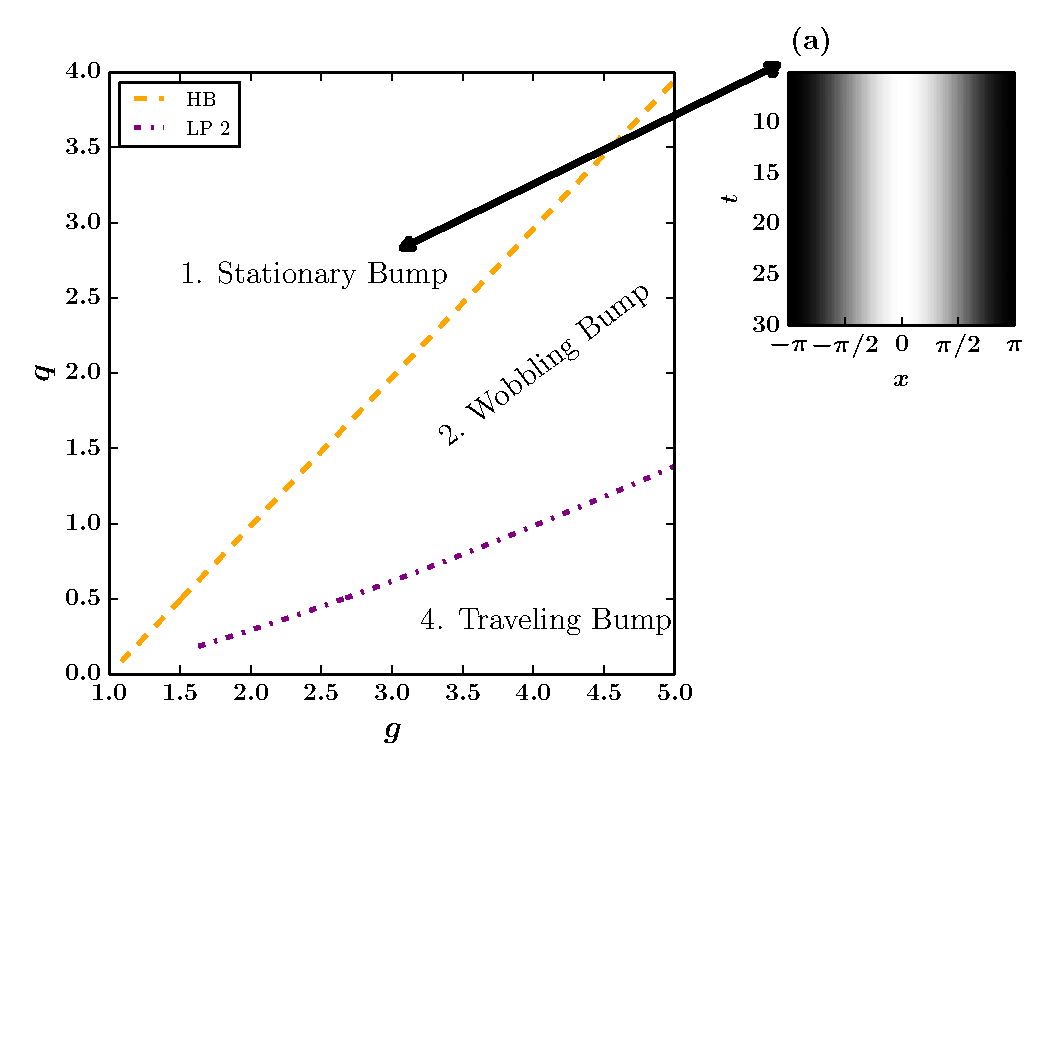
\includegraphics[width=.7\textwidth]{oned_full_2par1.pdf}
 %\caption{Bifurcation diagrams for the equivalent one-dimensional neural field model. Left: Bifurcation diagram over $g$ for fixed $q=0.5$. Right: Two parameter bifurcation diagram.}
\end{figure}
\end{frame}


\begin{frame}
\frametitle{Qualitative Dynamics on the 1D Domain}
\begin{figure}
 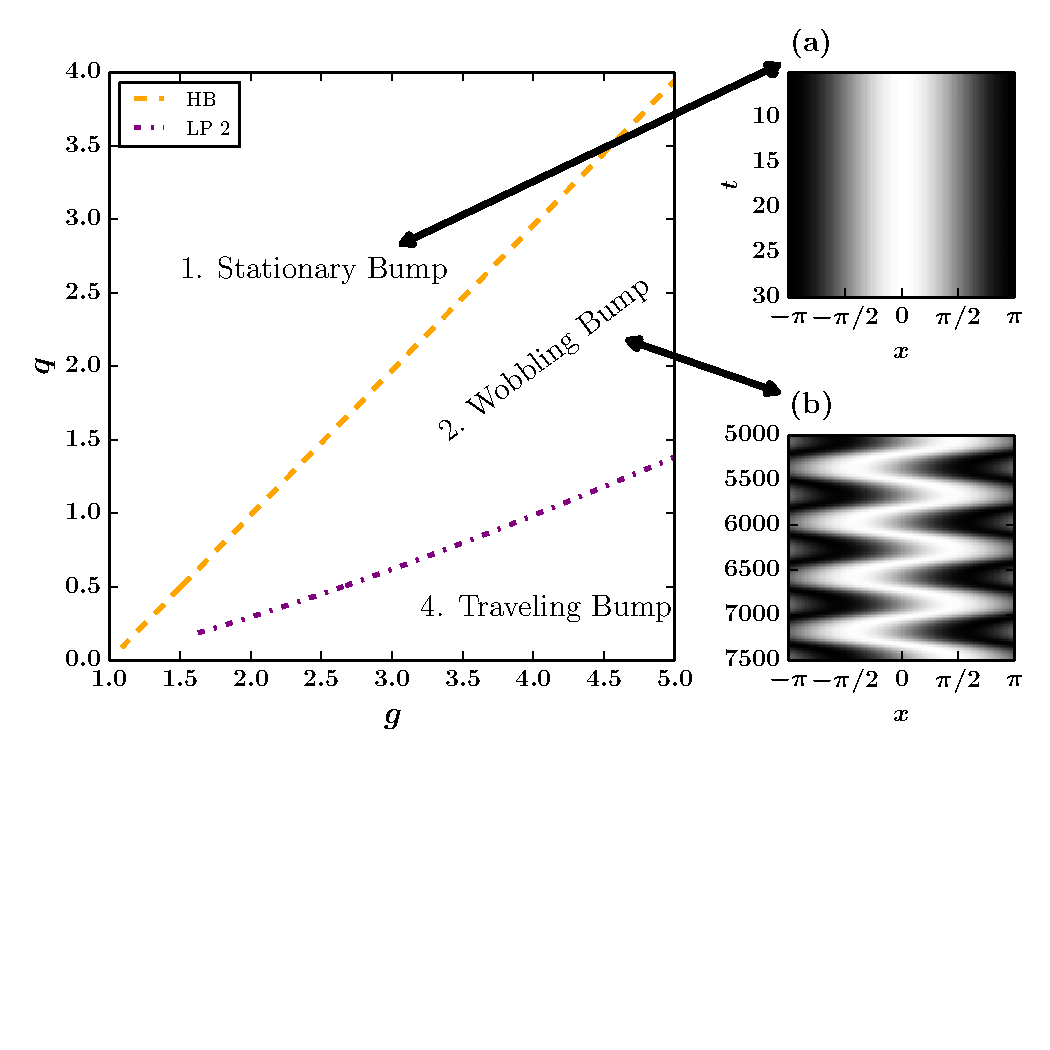
\includegraphics[width=.7\textwidth]{oned_full_2par2.pdf}
 %\caption{Bifurcation diagrams for the equivalent one-dimensional neural field model. Left: Bifurcation diagram over $g$ for fixed $q=0.5$. Right: Two parameter bifurcation diagram.}
\end{figure}
\end{frame}


\begin{frame}
\frametitle{Qualitative Dynamics on the 1D Domain}
\begin{figure}
 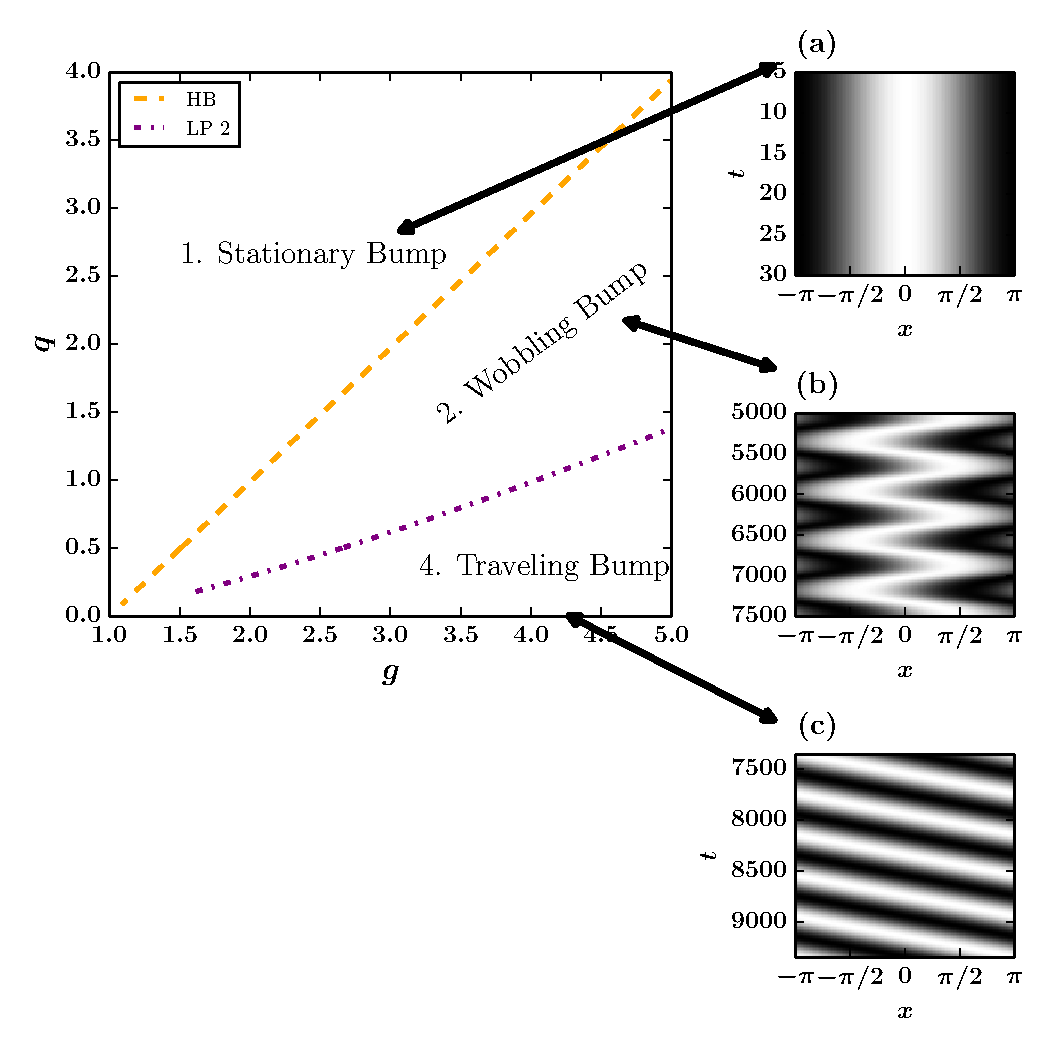
\includegraphics[width=.7\textwidth]{oned_full_2par3.pdf}
 %\caption{Bifurcation diagrams for the equivalent one-dimensional neural field model. Left: Bifurcation diagram over $g$ for fixed $q=0.5$. Right: Two parameter bifurcation diagram.}
\end{figure}
\end{frame}


\begin{frame}
\frametitle{Qualitative Dynamics on the 1D Domain}
\begin{figure}
 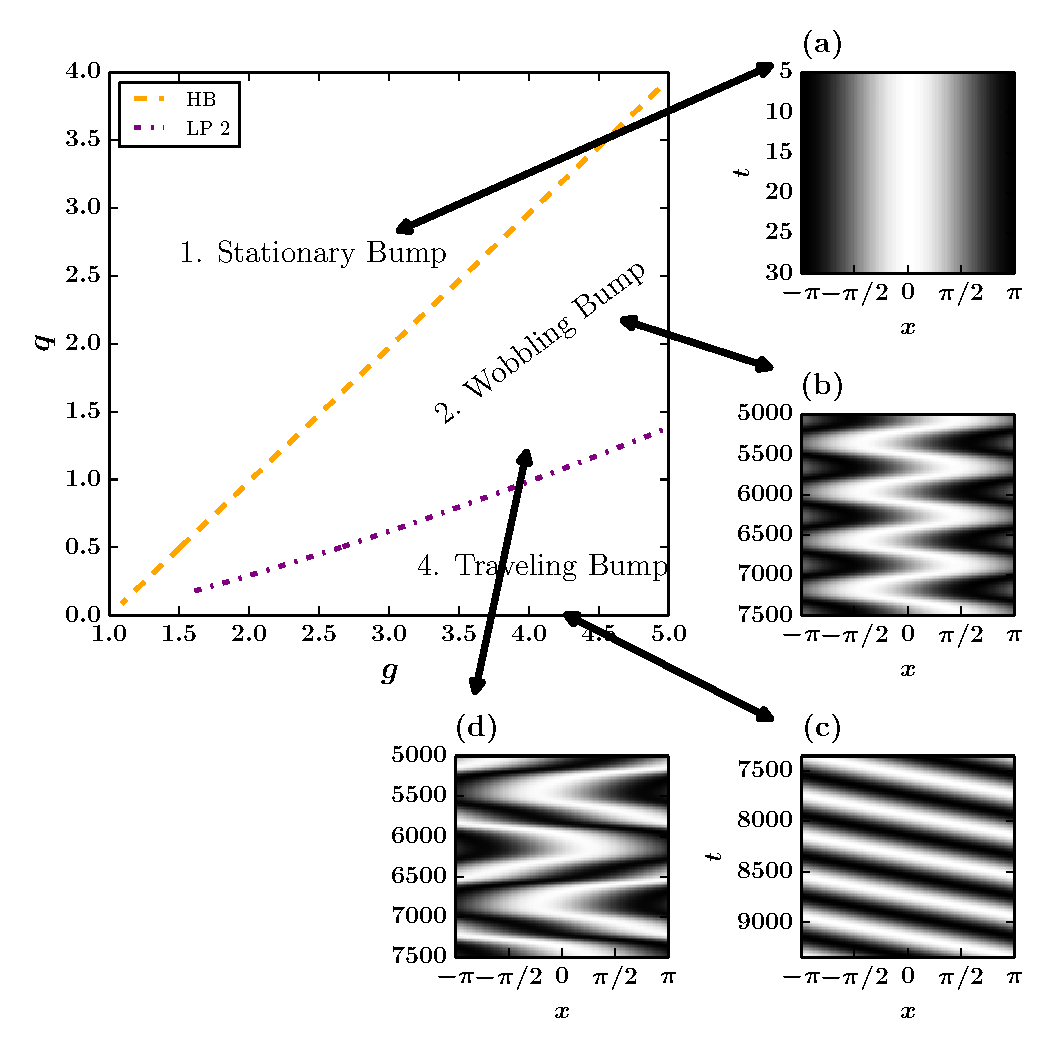
\includegraphics[width=.7\textwidth]{oned_full_2par4.pdf}
 %\caption{Bifurcation diagrams for the equivalent one-dimensional neural field model. Left: Bifurcation diagram over $g$ for fixed $q=0.5$. Right: Two parameter bifurcation diagram.}
\end{figure}
\end{frame}

\begin{frame}
\frametitle{Qualitative Dynamics on the 1D Domain}
\begin{figure}
 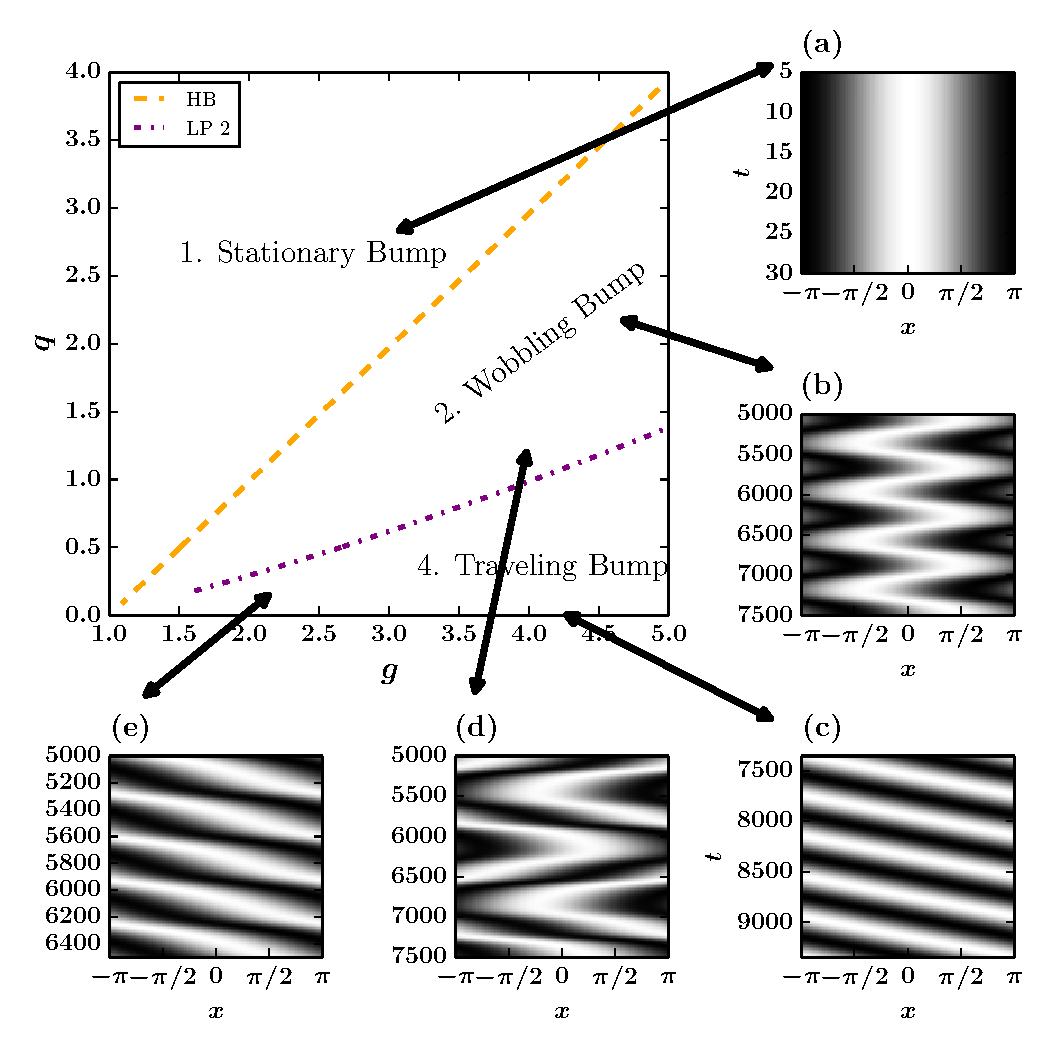
\includegraphics[width=.7\textwidth]{oned_full_2par5.pdf}
 %\caption{Bifurcation diagrams for the equivalent one-dimensional neural field model. Left: Bifurcation diagram over $g$ for fixed $q=0.5$. Right: Two parameter bifurcation diagram.}
\end{figure}
\end{frame}

\begin{frame}
\frametitle{One-dimensional Domain: Equivalent Phase Equation}
If $K(x) = A+B\cos(x)$, then $H(x) = \sin(x)$.
\begin{align*}
\frac{d\theta}{d\tau} &= qJ(\theta) -g\int_0^\tau e^{-(\tau-s)} H(\theta(s)-\theta(\tau))ds\\
&= -q\sin(\theta) -g [\cos(\theta)S(\tau) - \sin(\theta)C(\tau)],
\end{align*}
where
\begin{align*}
 S(\tau) = \int_0^\tau e^{-(\tau-s)} \sin\theta(s)ds, \quad C(\tau) = \int_0^\tau e^{-(\tau-s)} \cos\theta(s)ds
\end{align*}
\end{frame}

\begin{frame}
\frametitle{One-dimensional Domain: Equivalent Phase Equation}
So the phase model has equivalent form,
\begin{equation*}
\begin{split}
 \frac{d\theta}{d\tau} &= - q\sin(\theta) - g[\cos(\theta) S(\tau) - \sin(\theta) C(\tau)]\\
 \frac{dS}{d\tau} &= -S(\tau) + \sin\theta,\\
 \frac{dC}{d\tau} &= -C(\tau) + \cos\theta.
\end{split}
\end{equation*}
\end{frame}


\begin{frame}
\frametitle{Numerical Results on the 1D Domain: Phase Equation}
\begin{figure}
 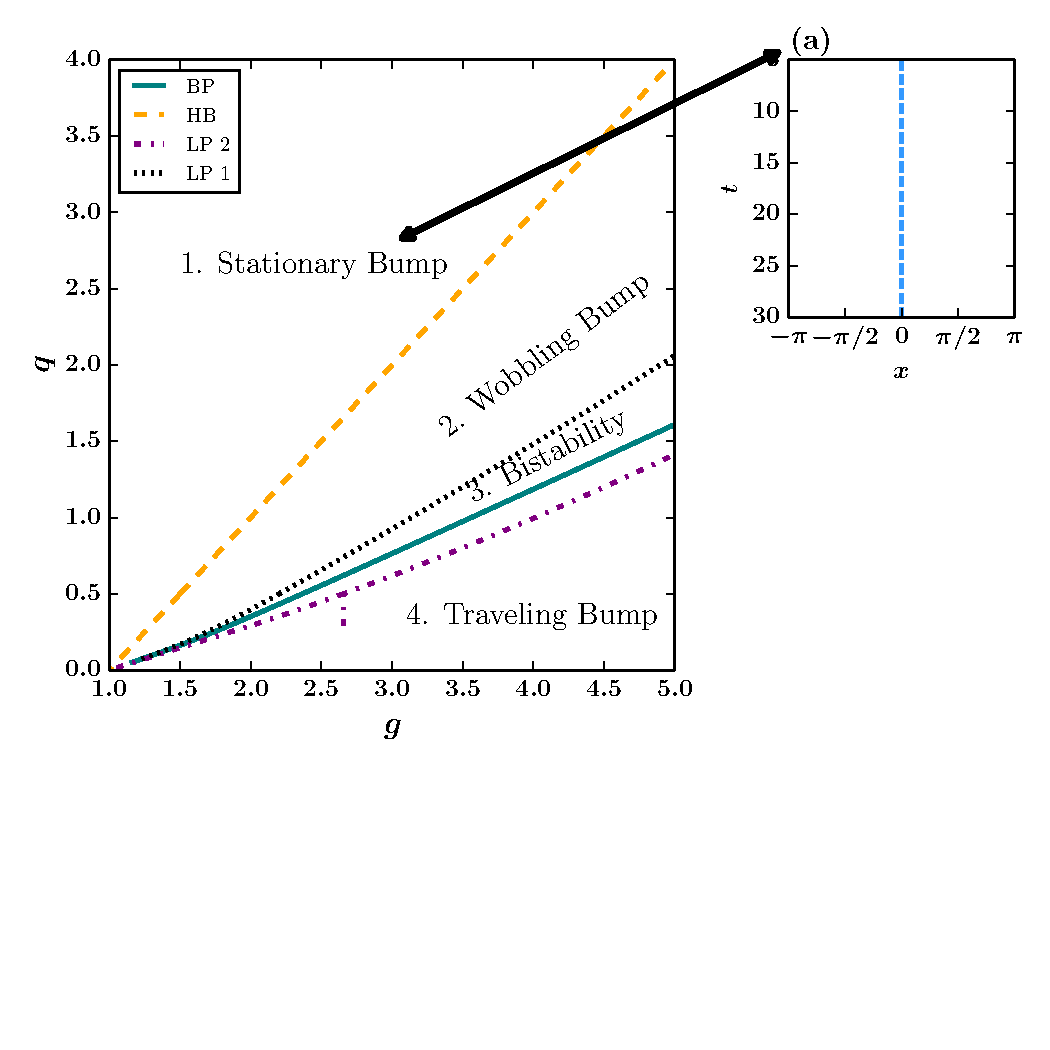
\includegraphics[width=.7\textwidth]{oned_phase_2par1.pdf}
 %\caption{Bifurcation diagrams for the equivalent one-dimensional phase model. Left: Bifurcation diagram over $g$ for fixed $q=0.5$. Right: Two parameter bifurcation diagram.}
\end{figure}
\end{frame}


\begin{frame}
\frametitle{Numerical Results on the 1D Domain: Phase Equation}
\begin{figure}
 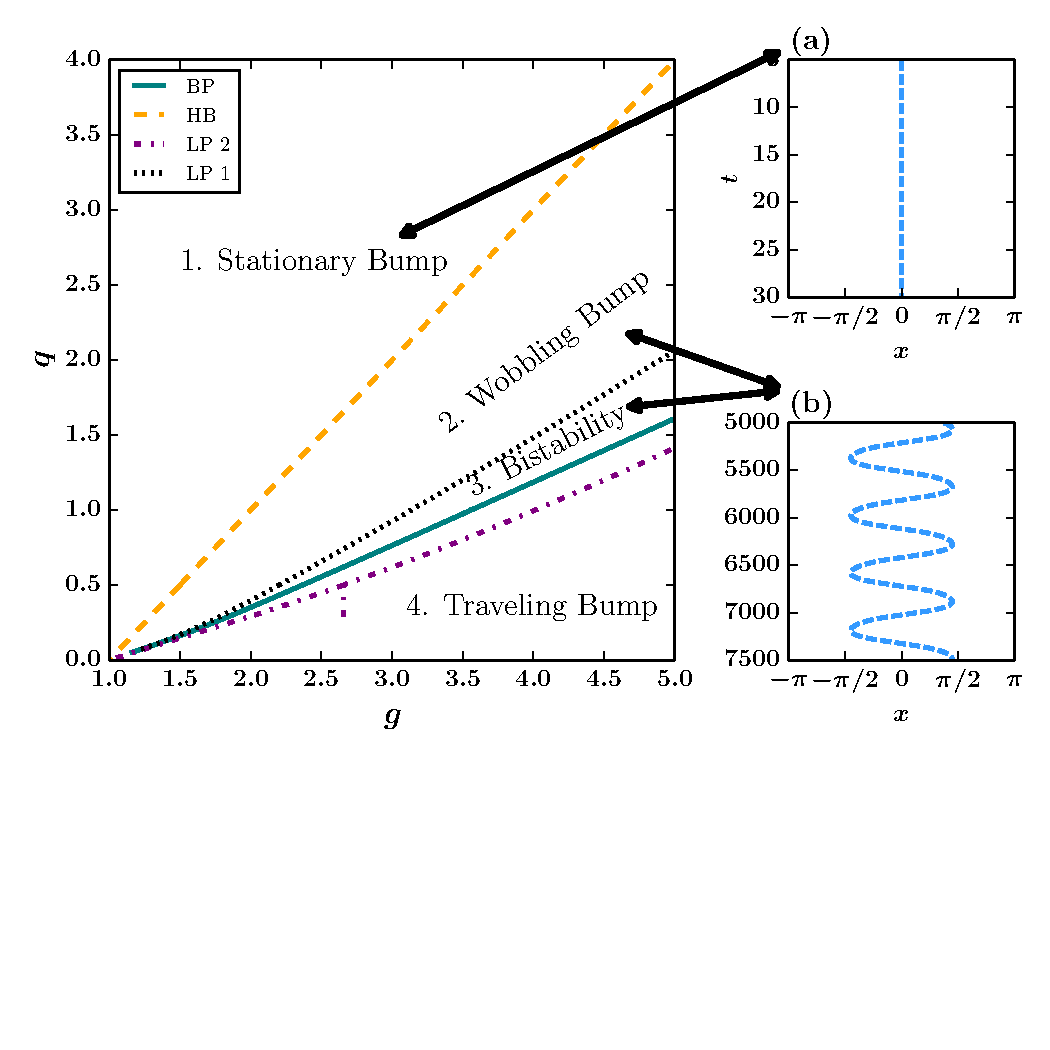
\includegraphics[width=.7\textwidth]{oned_phase_2par2.pdf}
 %\caption{Bifurcation diagrams for the equivalent one-dimensional phase model. Left: Bifurcation diagram over $g$ for fixed $q=0.5$. Right: Two parameter bifurcation diagram.}
\end{figure}
\end{frame}

\begin{frame}
\frametitle{Numerical Results on the 1D Domain: Phase Equation}
\begin{figure}
 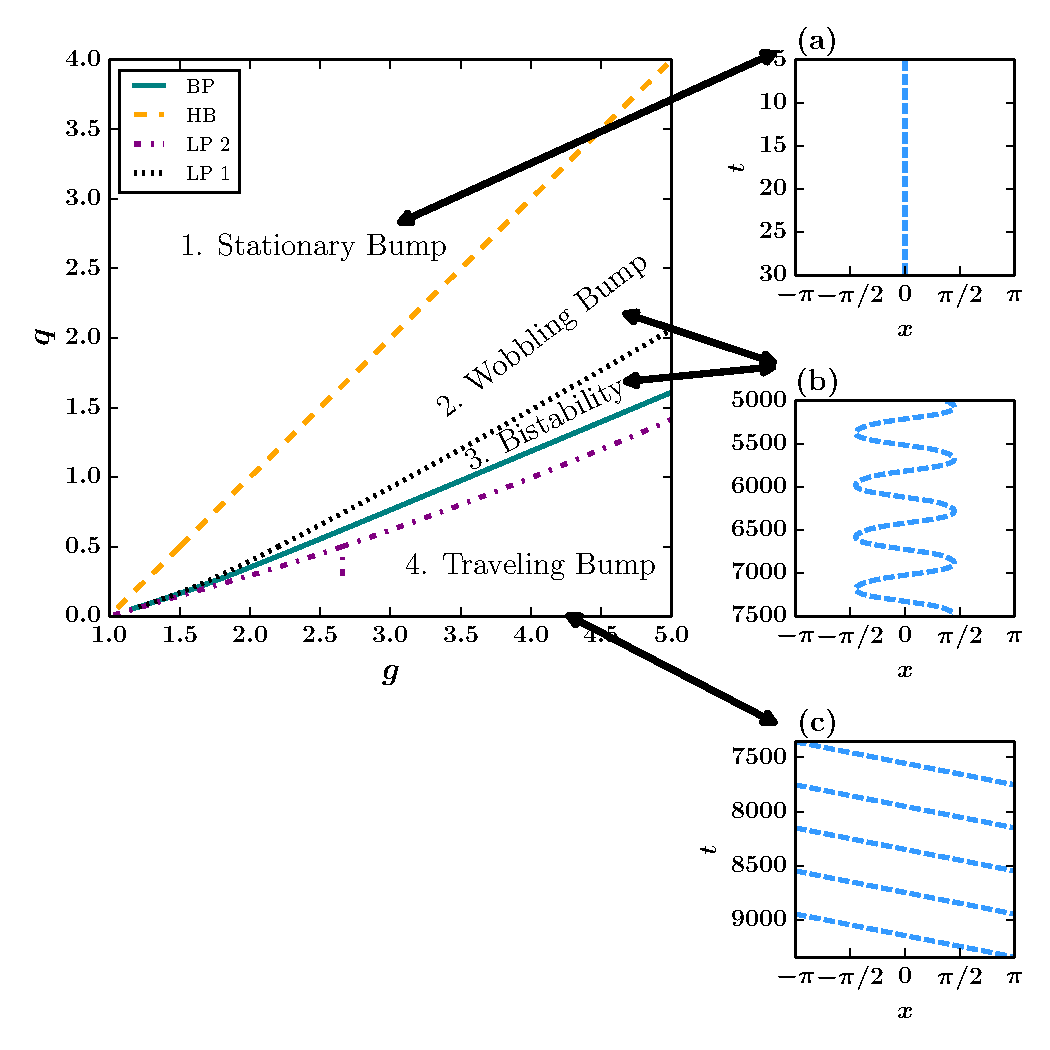
\includegraphics[width=.7\textwidth]{oned_phase_2par3.pdf}
 %\caption{Bifurcation diagrams for the equivalent one-dimensional phase model. Left: Bifurcation diagram over $g$ for fixed $q=0.5$. Right: Two parameter bifurcation diagram.}
\end{figure}
\end{frame}

\begin{frame}
\frametitle{Numerical Results on the 1D Domain: Phase Equation}
\begin{figure}
 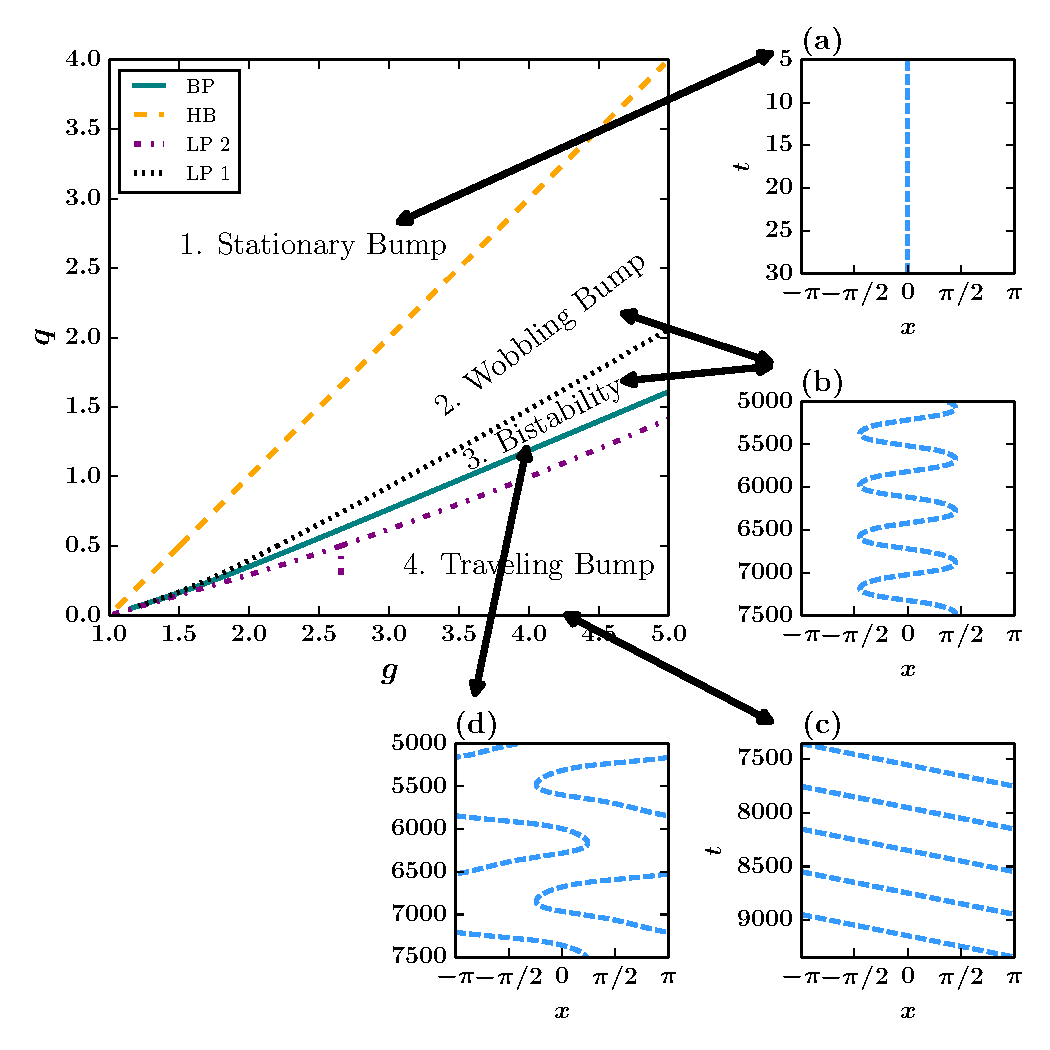
\includegraphics[width=.7\textwidth]{oned_phase_2par4.pdf}
 %\caption{Bifurcation diagrams for the equivalent one-dimensional phase model. Left: Bifurcation diagram over $g$ for fixed $q=0.5$. Right: Two parameter bifurcation diagram.}
\end{figure}
\end{frame}

\begin{frame}
\frametitle{Numerical Results on the 1D Domain: Phase Equation}
\begin{figure}
 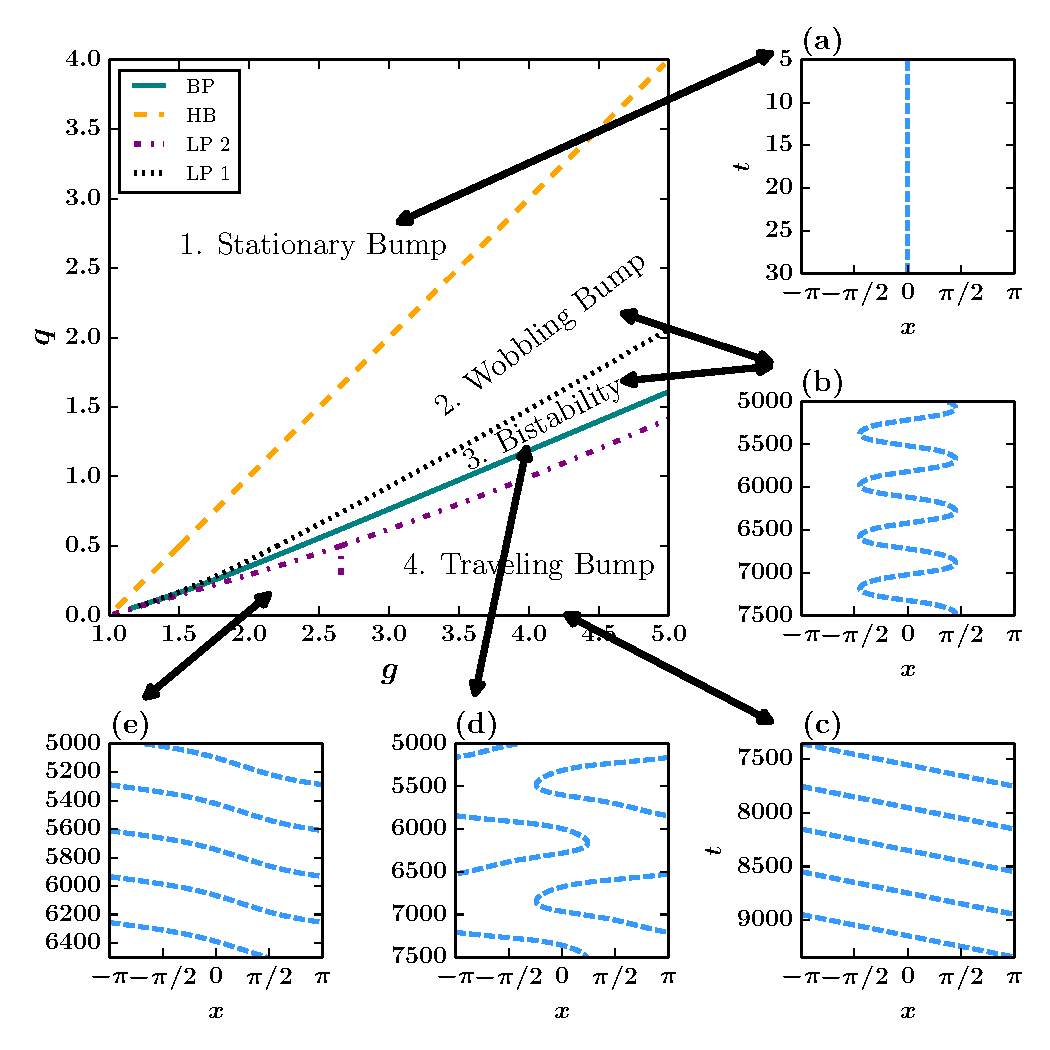
\includegraphics[width=.7\textwidth]{oned_phase_2par5.pdf}
 %\caption{Bifurcation diagrams for the equivalent one-dimensional phase model. Left: Bifurcation diagram over $g$ for fixed $q=0.5$. Right: Two parameter bifurcation diagram.}
\end{figure}
\end{frame}

\begin{frame}
\frametitle{Numerical Results on the 1D Domain: Phase Equation}
\begin{figure}
 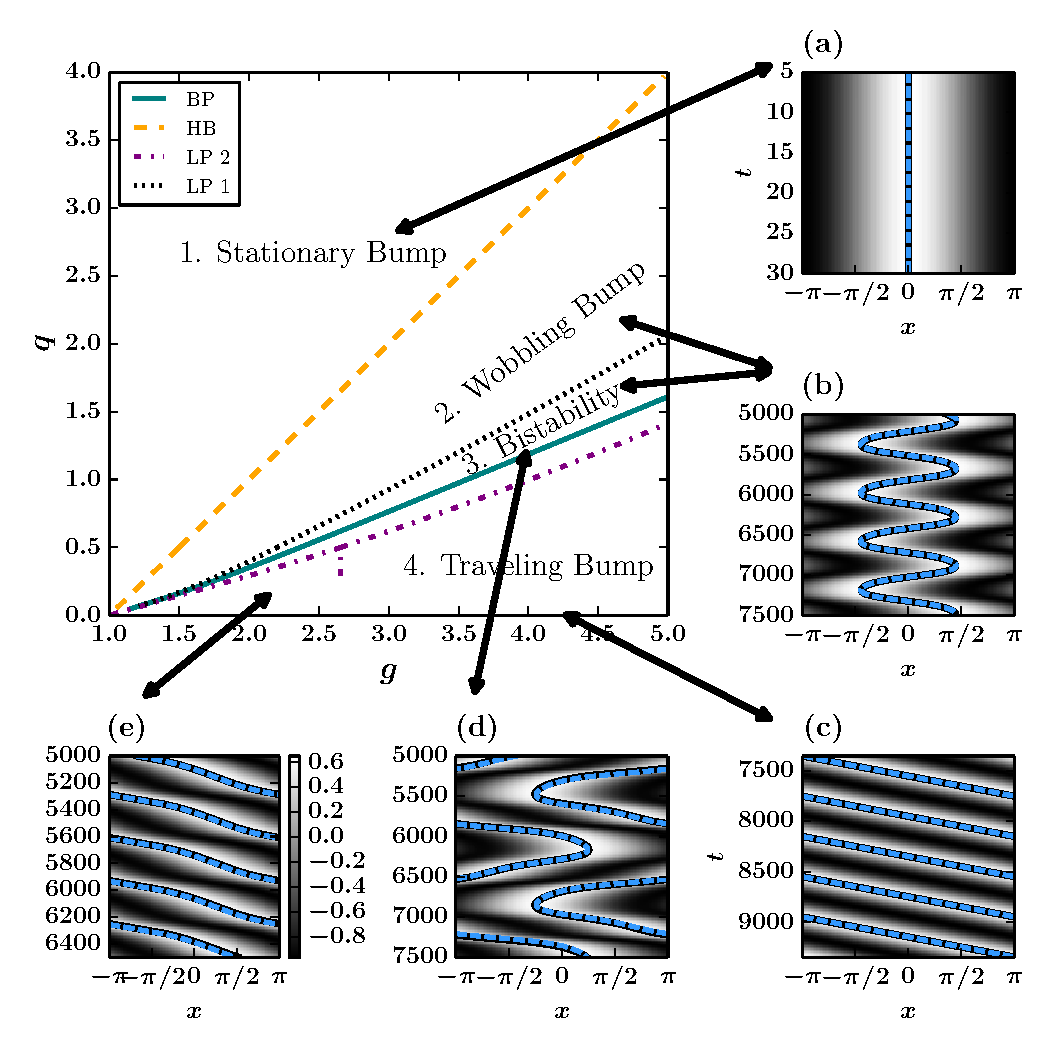
\includegraphics[width=.7\textwidth]{oned_phase_2par5b.pdf}
 %\caption{Bifurcation diagrams for the equivalent one-dimensional phase model. Left: Bifurcation diagram over $g$ for fixed $q=0.5$. Right: Two parameter bifurcation diagram.}
\end{figure}
\end{frame}

\begin{frame}
 \frametitle{Analytical Results on the 1D Domain: Oscillations}
 First, existence of a Hopf bifurcation:
 Let $\theta = 0 + \ve e^{\lambda \tau}$. Plug this expansion into the phase to get an equation for $\lambda$.
\begin{equation*}
\lambda^2 + \lambda[1-qJ'(0)-gH'(0)] - qJ'(0) = 0
\end{equation*}
Generally, $J'(0) < 0$ and $H'(0) > 0$, so there exists a Hopf bifurcation when
\begin{equation*}
 g^* = \frac{1-qJ'(0)}{H'(0)}.
\end{equation*}
with $q$ sufficiently large.

Existence and stability of oscillations follows from a normal form analysis.
\end{frame}

\begin{frame}
\frametitle{Analytical Results on the 1D Domain: Traveling Solutions}
Suppose $q=0$ and $g > 0$ and let $\theta(\tau) = \nu\tau$. Plugging in to the phase equation  with $H(x) = \sin(x)$ yields
\begin{align*}
 \nu &= -g \int_0^\infty e^{-s} H(-\nu s)ds\\
 &= g \int_0^\infty e^{-s} \sin(-\nu s)ds\\
 &= \frac{g\nu}{1+\nu^2}.
\end{align*}
So $\nu = \pm \sqrt{g-1}$
\end{frame}



\begin{frame}
 \frametitle{Conclusion of Analysis on the 1D domain}
 \begin{itemize}
  \item The phase model faithfully reproduces the dynamics of the neural field model
  \item The phase model allows for a much more straightforward analysis for the existence of particular dynamics
  \begin{itemize}
  \item Existence of sloshing solutions via a Hopf bifurcation.
  \item Stability of sloshing solutions via a normal form analysis.
  \item Existence of constant velocity traveling solutions.
  \item Existence and stability of non-constant velocity traveling solutions.
 \end{itemize}
\end{itemize}
\end{frame}

\subsection{Results on the Two-dimensional Domain}

\begin{frame}
\frametitle{Qualitative Dynamics on the Two-dimensional Domain}
We apply a similar transformation with the neural field model on two-dimensions.

\begin{itemize}
 \item<1-> Take a Fourier truncation of the kernel,
\begin{equation*}
 K(\x) = k_{00} + k_{10}\cos(x_1) + k_{01}\cos(x_2) + k_{11}\cos(x_1)\cos(x_2),
\end{equation*}
which allows us to rewrite the neural field equations on the 2D domain into a system of 18 ODEs.
 \item<2-> Although the numerics are more tractable and compatible with AUTO, we are unable to generate a two parameter bifurcation diagram.
\end{itemize}
\end{frame}

\begin{frame}
 \frametitle{2D Domain: Approximation of the Phase Equations}
  \begin{equation*}
\frac{d\theta_i}{d\tau} = qJ_i(\q) -g\int_0^\tau e^{-(\tau-s)} H_i(\q(s)-\q(\tau))ds, \quad i=1,2,
\end{equation*}
\begin{itemize}
 \item<1->  To generate bifurcation diagrams, we use the simplest nontrivial Fourier truncation of $H_i$,
\begin{equation*}
 H^F_1(\theta_1,\theta_2) =  \sin(\theta_1)(h_{10} + h_{11}\cos(\theta_2)).
\end{equation*}
\item<2-> We can then rewrite the phase equations as a system of 10 ODEs and generate bifurcation diagrams using AUTO.
\end{itemize}

\end{frame}

%\begin{frame}
%\frametitle{Results on the Two-dimensional Domain: Approximation of the Phase Equations}
%\begin{figure}
% 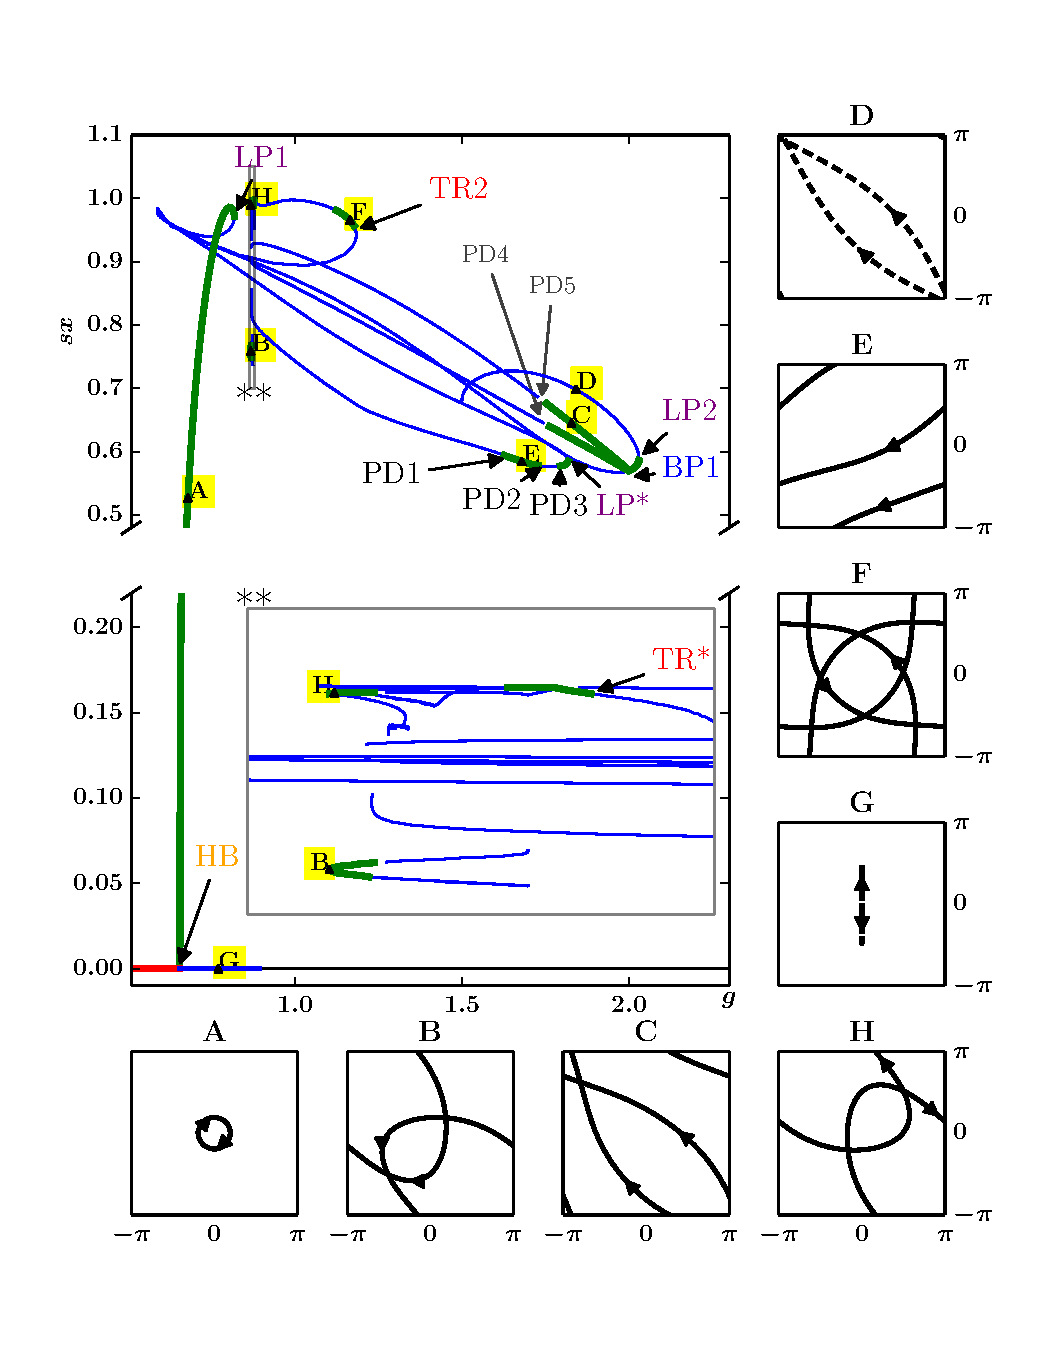
\includegraphics[width=.6\textwidth]{twod_phase_auto_3terms_q=0p1.pdf}
% \caption{}
%\end{figure}
%\end{frame}

\begin{frame}
\frametitle{Numerical Results on the 2D Domain: Phase Equation}
\begin{figure}
 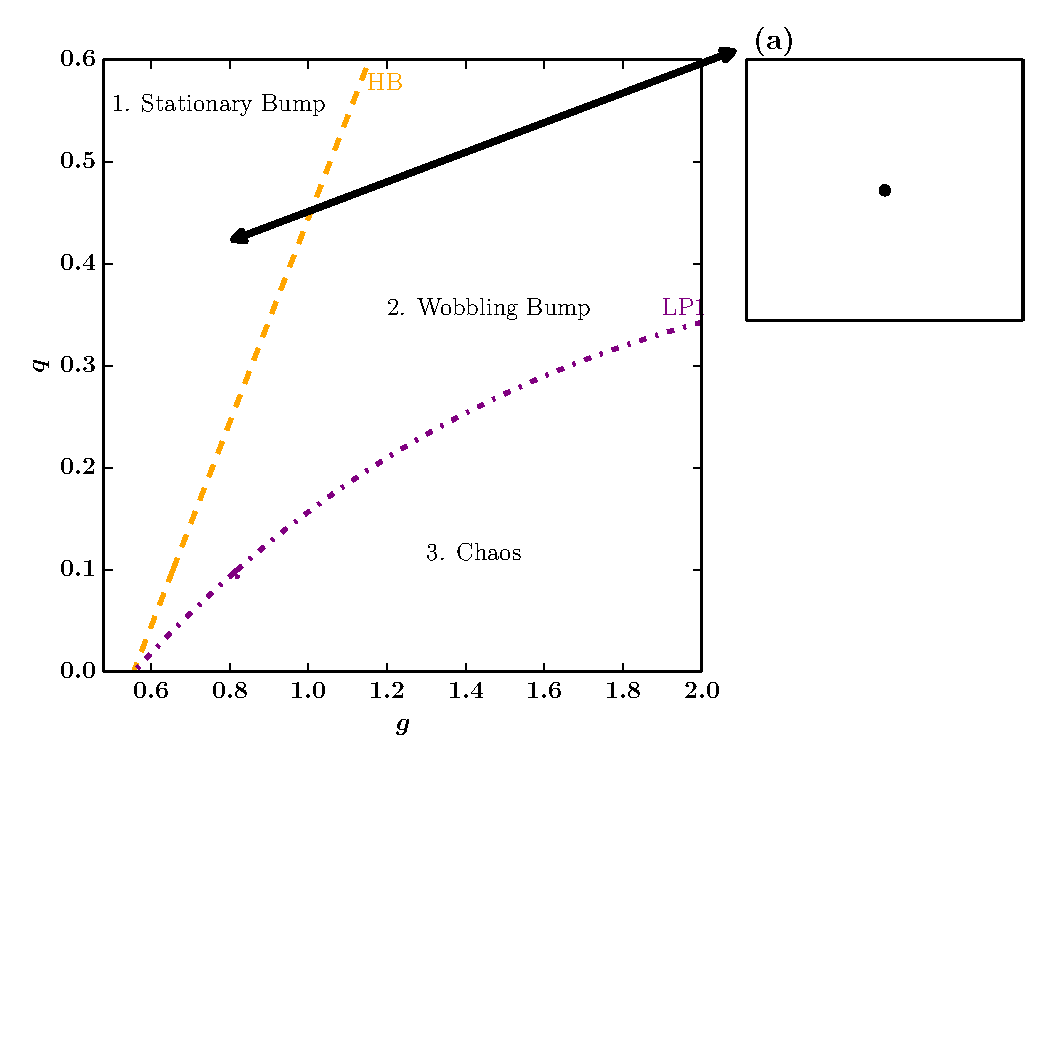
\includegraphics[width=.6\textwidth]{twod_phase_2par1.pdf}

\end{figure}
\end{frame}

\begin{frame}
\frametitle{Numerical Results on the 2D Domain: Phase Equation}
\begin{figure}
 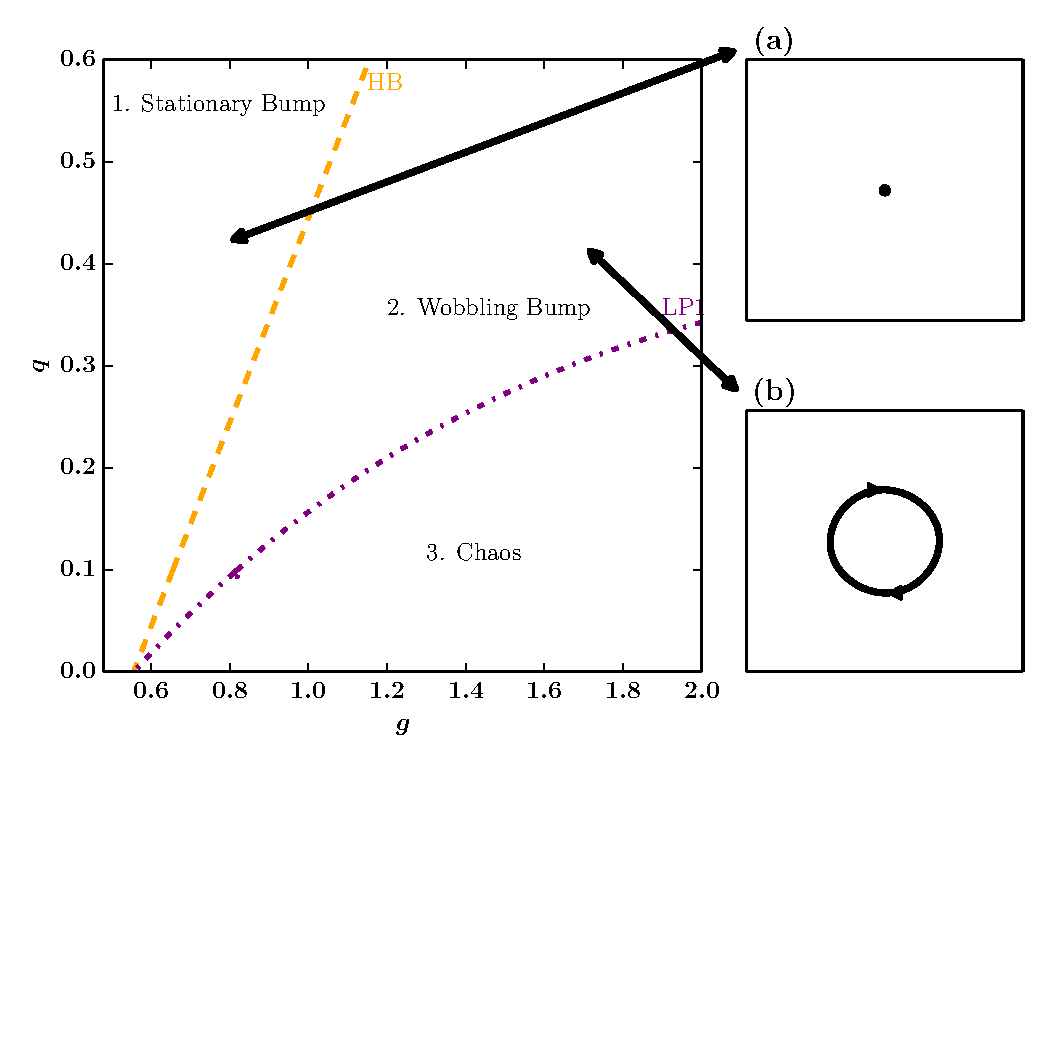
\includegraphics[width=.6\textwidth]{twod_phase_2par2.pdf}

\end{figure}
\end{frame}

\begin{frame}
\frametitle{Numerical Results on the 2D Domain: Phase Equation}
\begin{figure}
 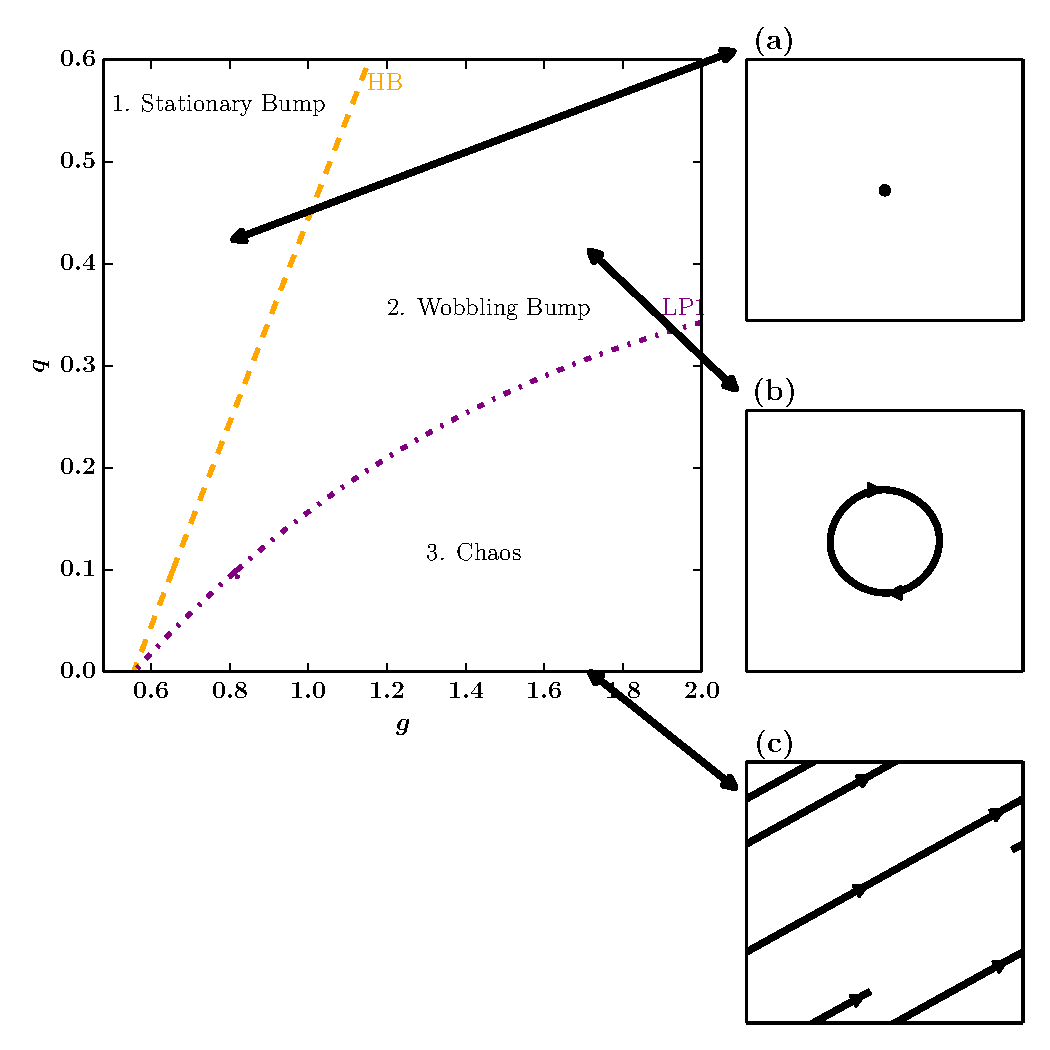
\includegraphics[width=.6\textwidth]{twod_phase_2par3.pdf}

\end{figure}
\end{frame}

\begin{frame}
\frametitle{Numerical Results on the 2D Domain: Phase Equation}
\begin{figure}
 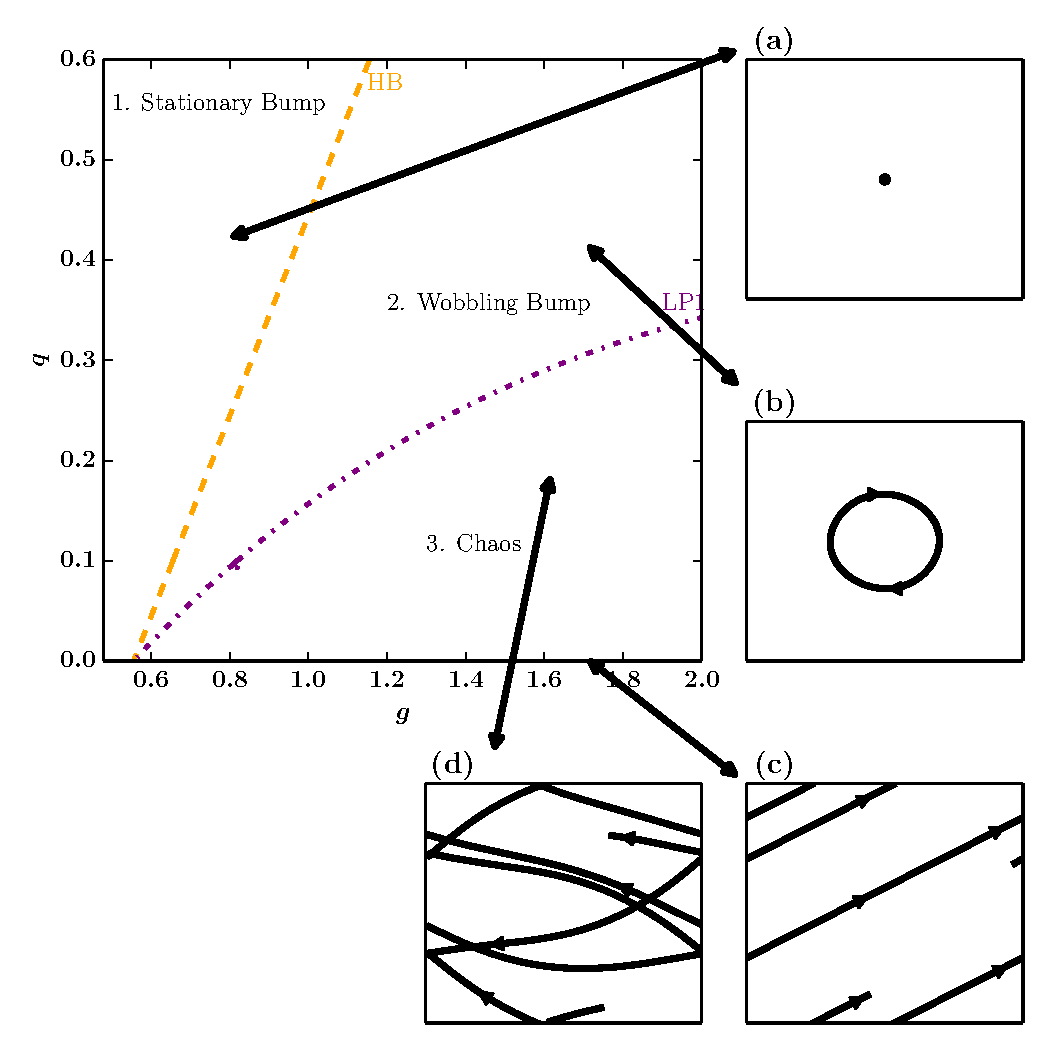
\includegraphics[width=.6\textwidth]{twod_phase_2par4.pdf}

\end{figure}
\end{frame}

\begin{frame}
\frametitle{Numerical Results on the 2D Domain: Phase Equation}
\begin{figure}
 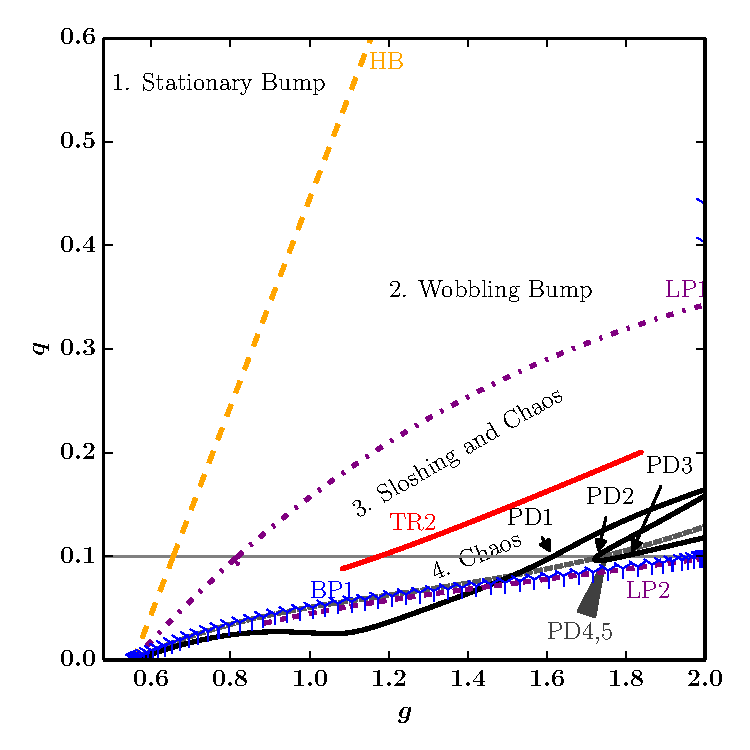
\includegraphics[width=.6\textwidth]{twod_phase_auto_3terms_2par.pdf}

\end{figure}
\end{frame}



\begin{frame}
\frametitle{Analytical Results on the 2D Domain}
Let $q=0$ and consider the ansatz $\theta_1(\tau) = \nu_1\tau$ and $\theta_2(\tau) = \nu_2\tau$. Constant velocity bump solutions exist if $\nu_1,\nu_2$ simultaneously satisfy
\begin{equation*}
\begin{split}
 \nu_1 &=  g \int_0^\infty e^{-s} H_1(\nu_1 s,\nu_2 s) ds,\\
 \nu_2 &=  g \int_0^\infty e^{-s} H_2(\nu_1 s,\nu_2 s) ds.
\end{split}
\end{equation*}
If we take $H_i = H_i^F$, we can solve for $\nu_1,\nu_2$ explicity.
\end{frame}


\begin{frame}
\frametitle{Analytical Results on the 2D Domain: Constant Velocity Solutions (Existence)}
\begin{figure}
 \centering
 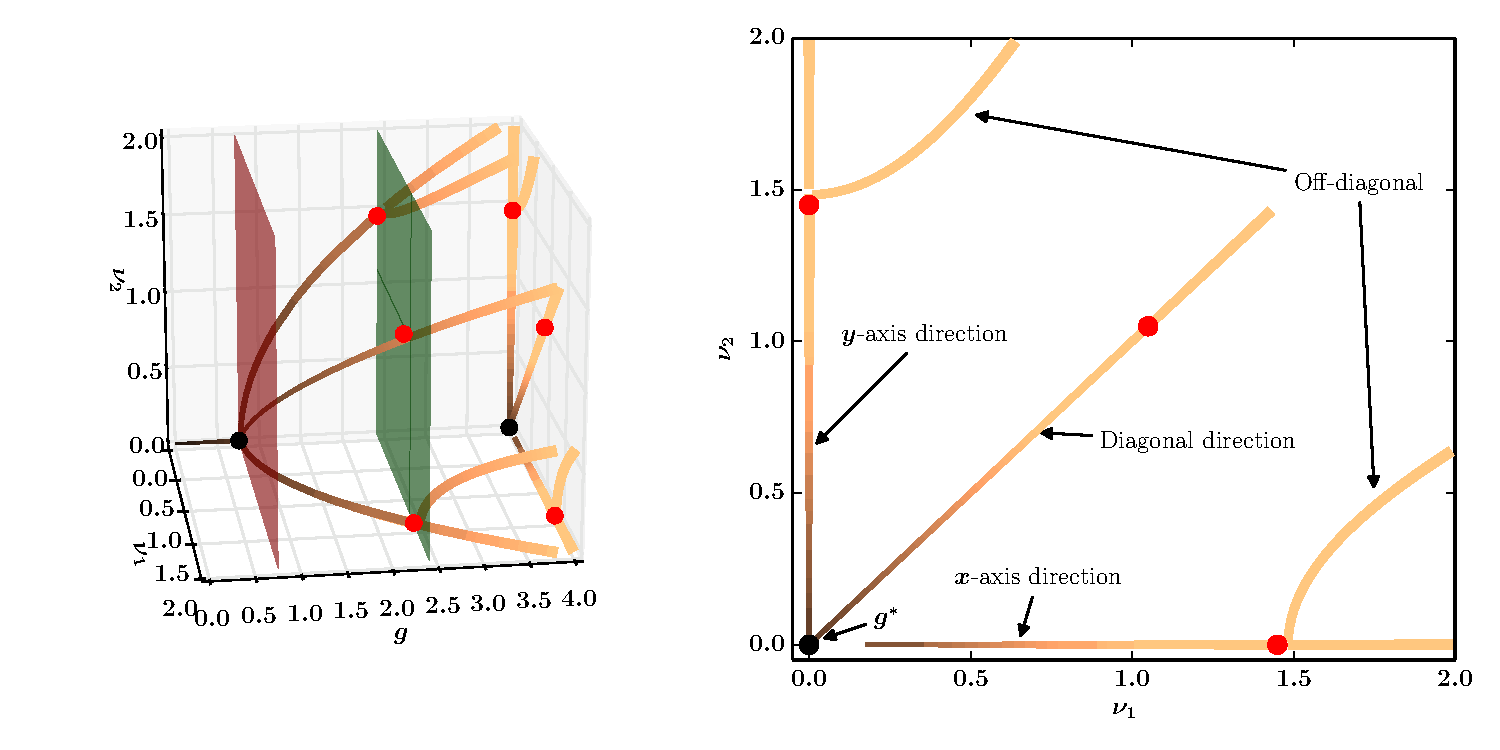
\includegraphics[width=.7\textwidth]{twod_wave_exist_trunc_v4.pdf}
 \caption{Existence of traveling bump solutions using the truncated interaction function $H_i^F$.}

 \end{figure}
\end{frame}



\begin{frame}
 \frametitle{Conclusion of Analysis on the 2D domain}
 \begin{itemize}
  \item The phase model qualitatively reproduces the dynamics of the neural field model.
  \item As in the 1D domain, the phase model allows for a much more straightforward analysis for the existence of particular dynamics
  \begin{itemize}
  \item Existence of sloshing solutions via a Hopf bifurcation.
  \item Existence of constant velocity traveling solutions.
  \item Existence and stability of non-constant velocity traveling solutions.
 \end{itemize}
\end{itemize}
\end{frame}


\section{Conclusion}
\begin{frame}
 \frametitle{Conclusion}
 \vspace{-.1in}
 \begin{itemize}
  \item We successfully reduce the dimensionality of the model to one or two scalar differential equations representing the coordinates of the centroid.
  \item This reduction places no strong assumptions on the firing rate function or the kernel.
  \item Using this reduction, we show that it faithfully reproduces the dynamics of the original neural field model, and we use it to rigorously classify the existence and stability of various bump dynamics.
 \end{itemize}'

% \begin{figure}
%  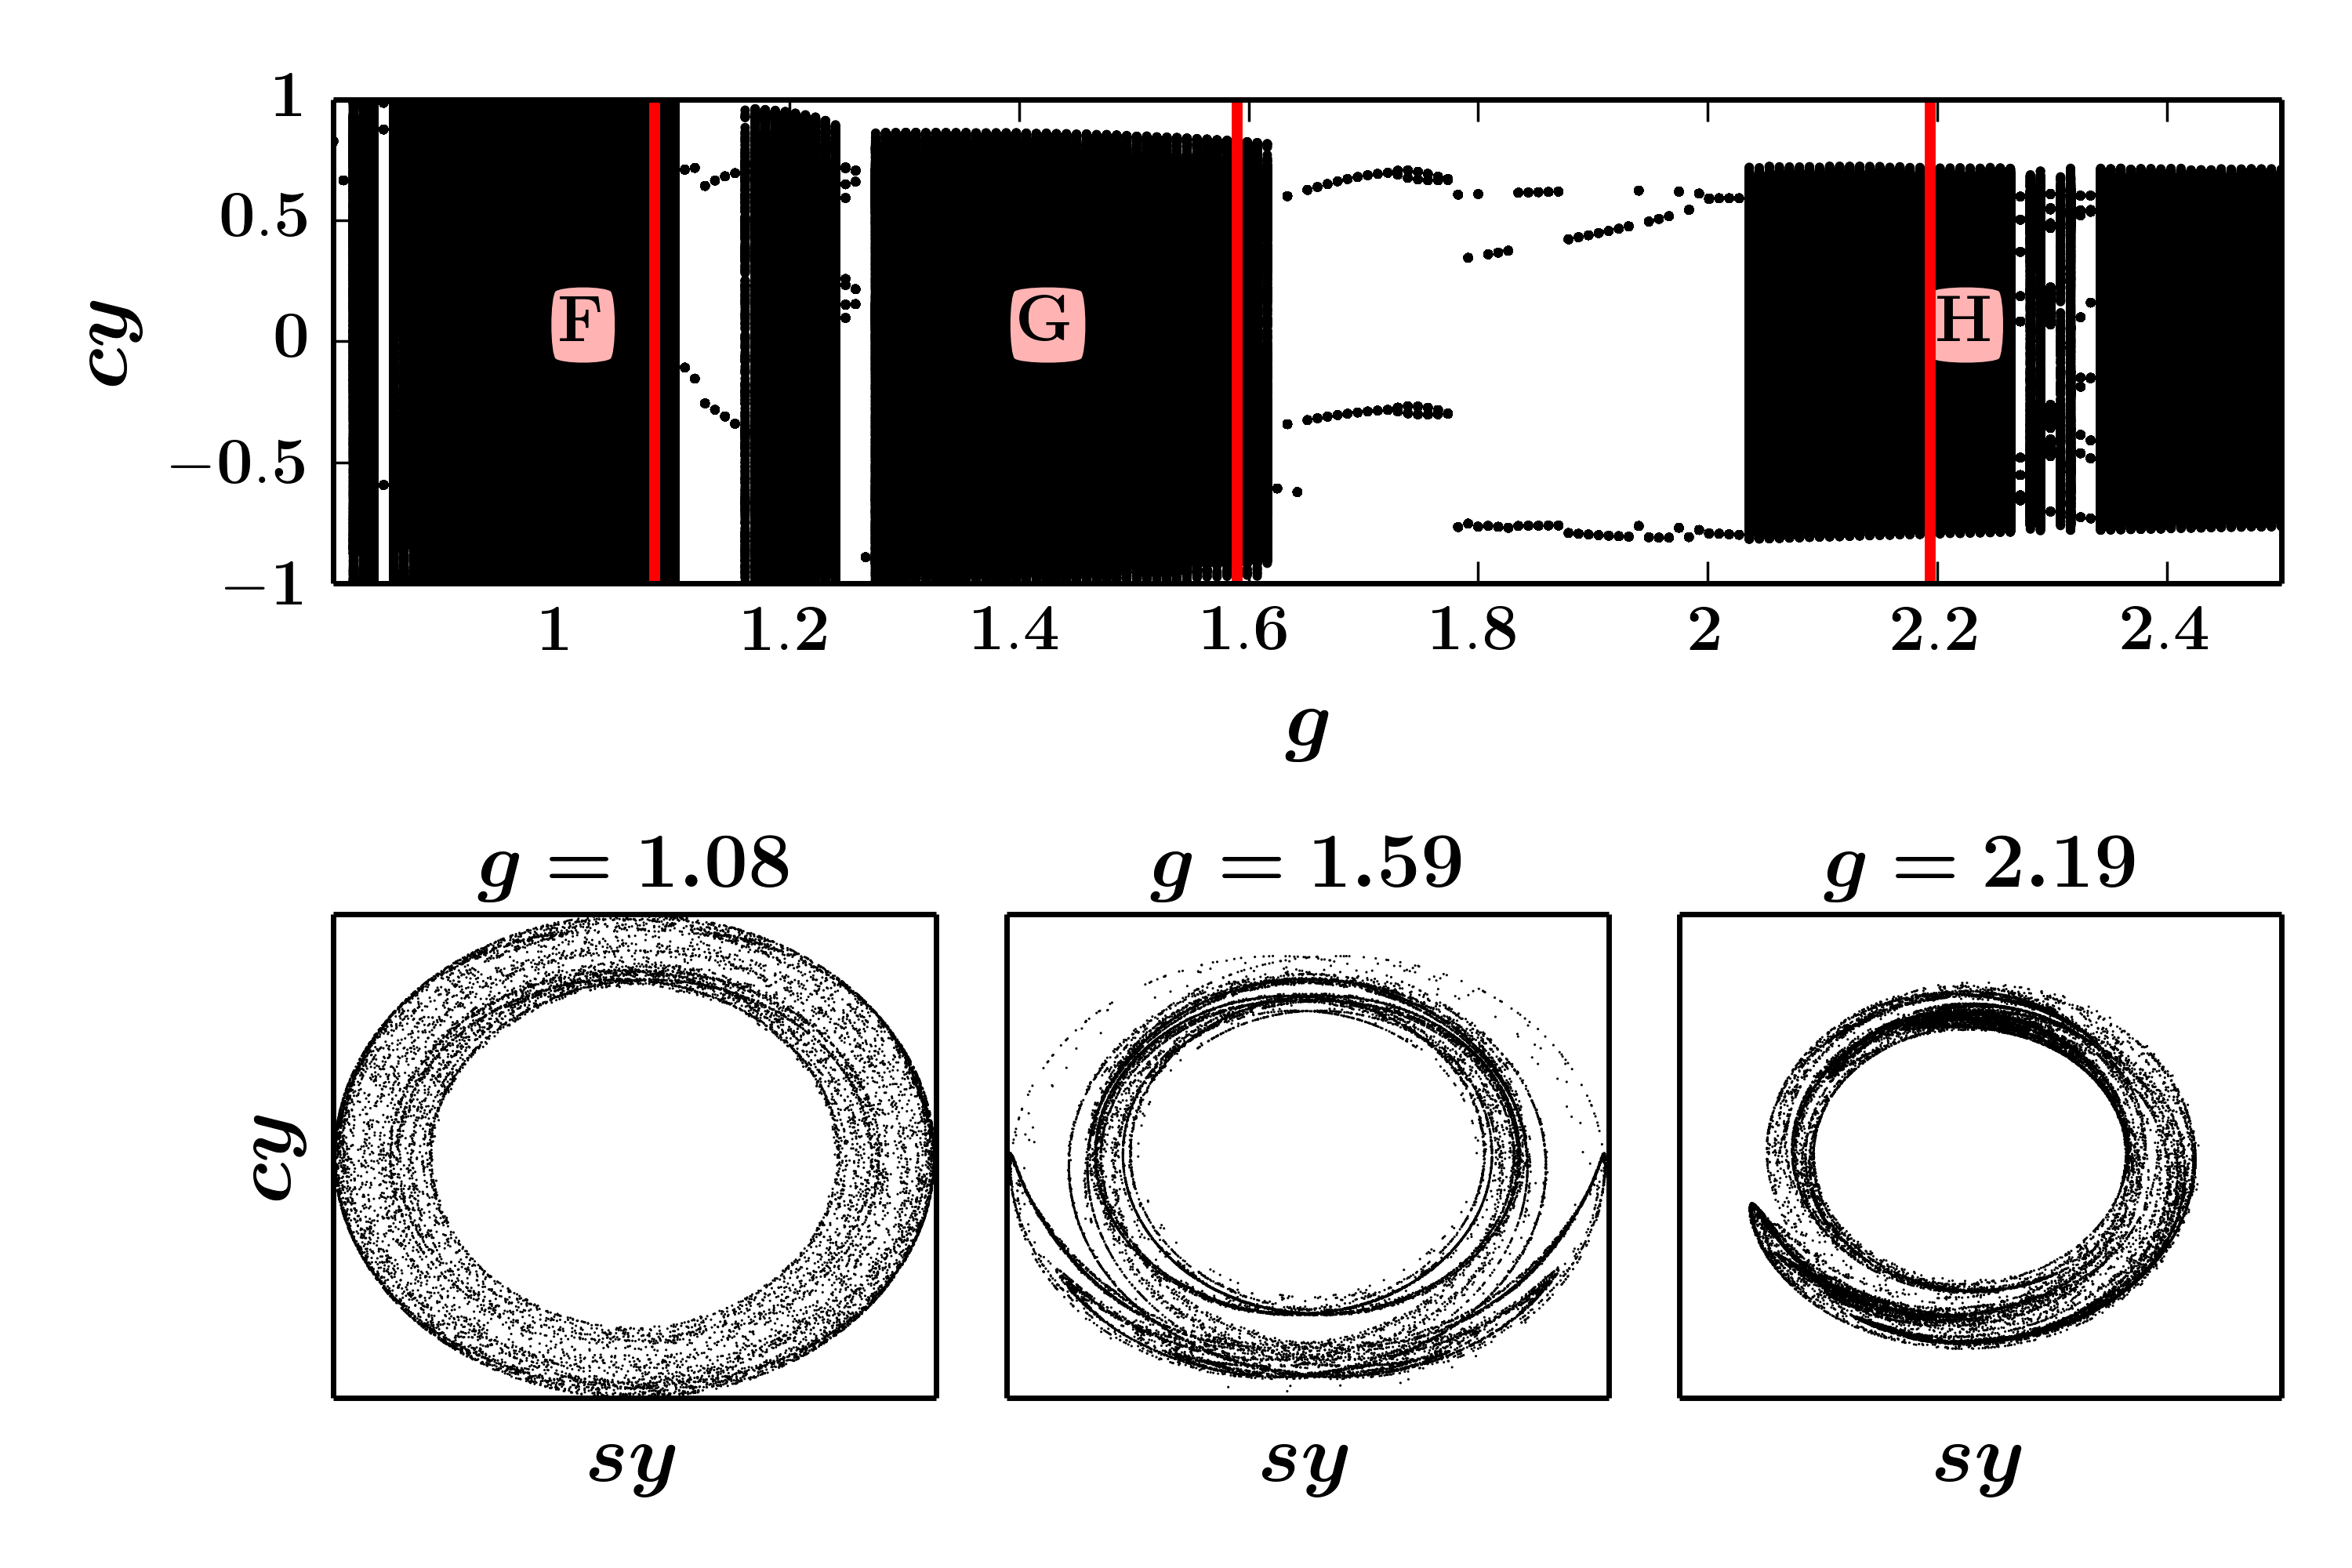
\includegraphics[width=.45\textwidth]{twod_phase_3terms_chaos_fig.png}
% \end{figure}

\end{frame}


\begin{frame}[noframenumbering]
 \frametitle{Acknowledgements}
 
 \begin{columns}
\begin{column}{0.5\textwidth}
\begin{itemize}
  \item NSF DMS 1712922
  \item Kreso Josic
 \item Zack Kilpatrick
 \item Josh Gold
 \item G. Bard Ermentrout
%   \begin{figure}
%    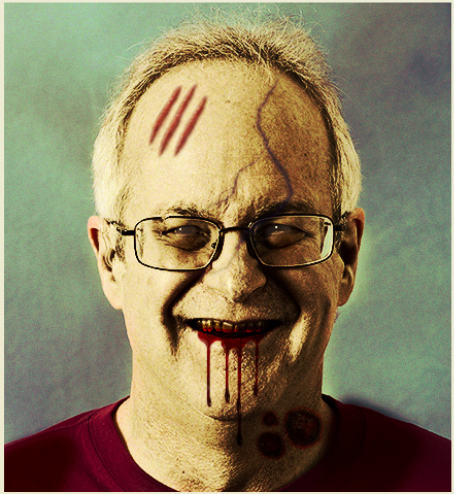
\includegraphics[width=.6\textwidth]{zombie_bard.png}
%   \end{figure}
  \end{itemize}
  
\end{column}
\begin{column}{0.5\textwidth}  %%<--- here
 Thanks to members of the Pitt math bio group
 \begin{itemize}
 \item Jon Rubin
 \item Brent Doiron
 \item Abby Pekoske
 \item Marcello Codiani
 \item Jay Pina
  \end{itemize}
  and visiting scholars
 \begin{itemize}
  \item Cati Vich (Universitat De Les Illes Balears)
  \item Aki Akao (Univ. of Tokyo)
 \end{itemize}



\end{column}
\end{columns}
 

\end{frame}



\begin{frame}[allowframebreaks]
 \bibliographystyle{plain}
\bibliography{../../../youngmin-bard/ymp,../../../youngmin-bard/neuralfield,../../../youngmin-bard/bio,audio}{}
\end{frame}



\section{Appendix}




\end{document}








\begin{frame}
\frametitle{Qualitative Dynamics on the One-dimensional Domain}
Recall the neural field model, this time on a 1D domain:
\begin{eqnarray*}
\frac{\partial u(x,t)}{\partial t} &=& -u(x,t) + \int_0^{2\pi} K(x-y) f(u(y,t))\ dy  \\
{} &+& \ve \left[q I(x) - g z(x,t)\right] \nonumber, \\
\label{eq:z1}
\frac{\partial z(x,t)}{\partial t} &=& \ve [-z(x,t)+u(x,t)],
\end{eqnarray*}
\end{frame}







\begin{frame}
\frametitle{Qualitative Dynamics on the 2D Domain}
\begin{figure}
 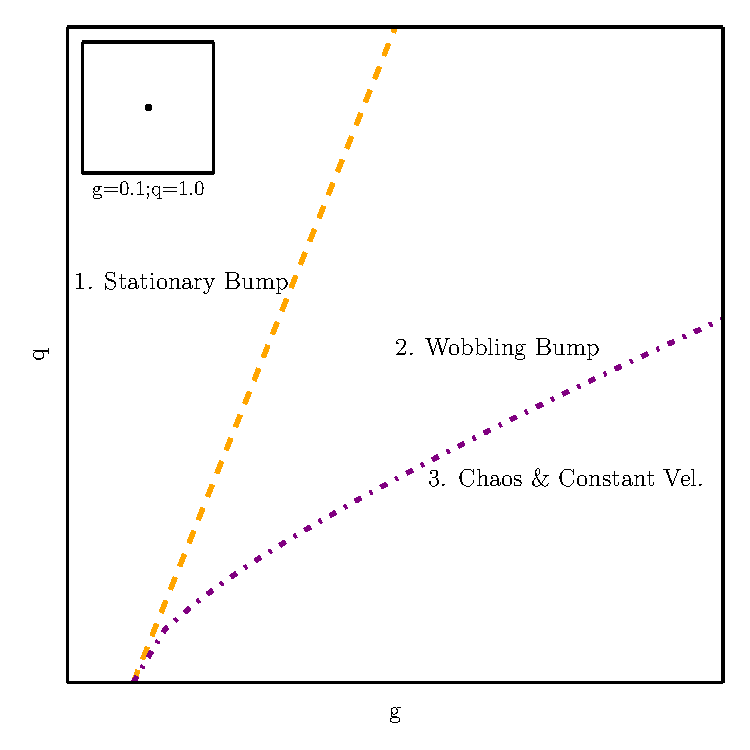
\includegraphics[width=.77\textwidth]{twod_full_auto_5terms_2par1.pdf}
 \caption{}
\end{figure}
\end{frame}

\begin{frame}
\frametitle{Qualitative Dynamics on the 2D Domain}
\begin{figure}
 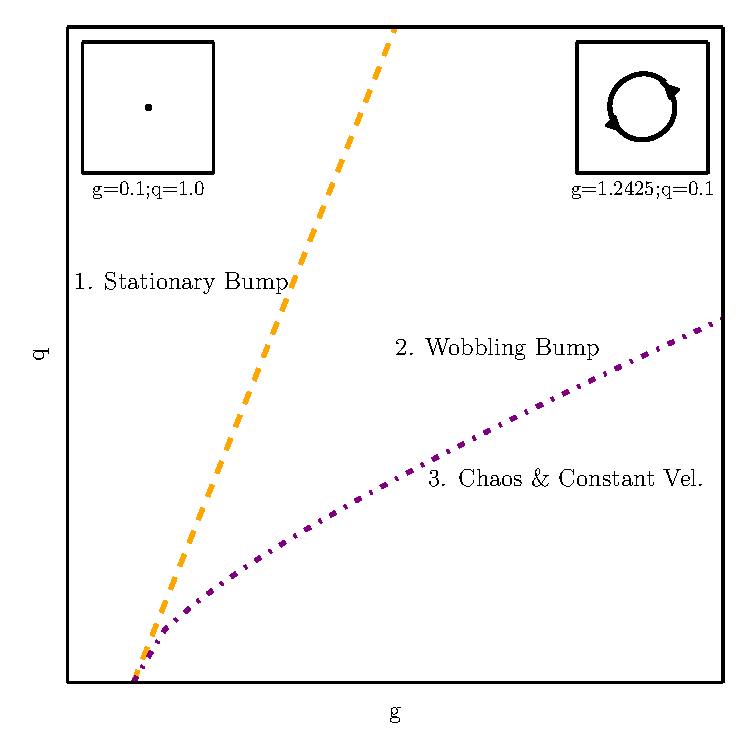
\includegraphics[width=.77\textwidth]{twod_full_auto_5terms_2par2.pdf}
 \caption{}
\end{figure}
\end{frame}

\begin{frame}
\frametitle{Qualitative Dynamics on the 2D Domain}
\begin{figure}
 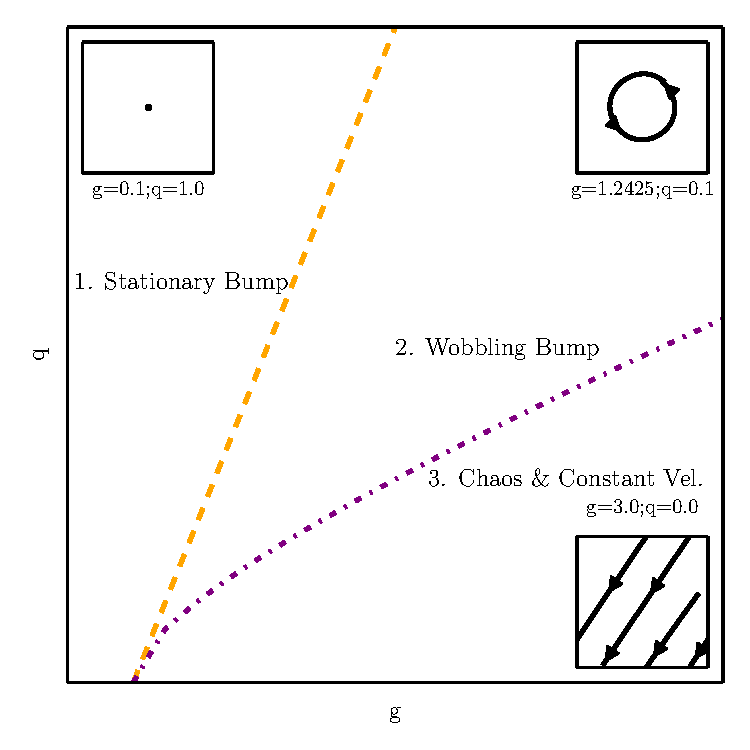
\includegraphics[width=.77\textwidth]{twod_full_auto_5terms_2par3.pdf}
 \caption{}
\end{figure}
\end{frame}


\begin{frame}
\frametitle{Qualitative Dynamics on the 2D Domain}
\begin{figure}
 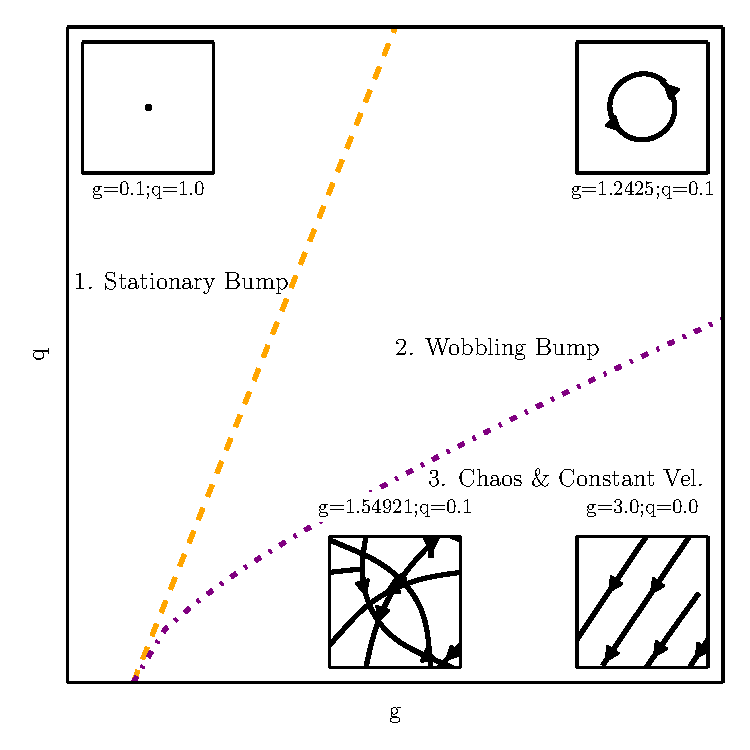
\includegraphics[width=.77\textwidth]{twod_full_auto_5terms_2par4.pdf}
 \caption{}
\end{figure}
\end{frame}

